\chapter{Database Design}
\label{chap:database-design}

\section{Introduction}
The database architecture serves as the foundation for data persistence, transactional integrity, and workspace isolation in the Nexus PM platform. As a decoupled SaaS application, Nexus PM relies on a structured relational database schema to guarantee ACID properties (Atomicity, Consistency, Isolation, Durability) across collaborative workflows. 

The role of the database design is to enforce business-level constraints directly within the storage engine, optimize query execution paths, and secure tenant separation. This chapter outlines the physical schema, entity relationships, database constraints, indexing strategies, and schema migration workflows.

\section{Database Technology}
Nexus PM utilizes \textbf{PostgreSQL} as its primary database engine, hosted via the managed \textbf{Supabase} cloud platform. PostgreSQL was selected based on several architectural criteria:
\begin{itemize}
    \item \textbf{Relational Model Robustness:} The core entity structures (Workspaces, Projects, Members, Tasks) are highly relational. PostgreSQL provides rigid foreign key constraints, unique constraints, and check conditions that prevent data anomalies.
    \item \textbf{ACID Compliance:} Operations such as token generation, project membership updates, and task assignments require transaction guarantees. PostgreSQL ensures that either all steps commit successfully or the transaction is rolled back.
    \item \textbf{PgBouncer Connection Pooling:} Managed hosting on Supabase includes a pre-configured PgBouncer instance running in transaction-pooling mode. This maps incoming transient client connections to a smaller pool of persistent database connections, preventing connection exhaustion under high API concurrent loads.
    \item \textbf{Reliability and Backups:} The managed database service automates daily snapshot backups, handles security updates, and provides physical replication points, minimizing operational maintenance.
\end{itemize}

\section{Entity Relationship Model}
The database schema is organized around the User, Project, and Task entities. Figure~\ref{fig:database_erd} shows the layout of the primary tables and their relationships.

\begin{figure}[h!]
    \centering
    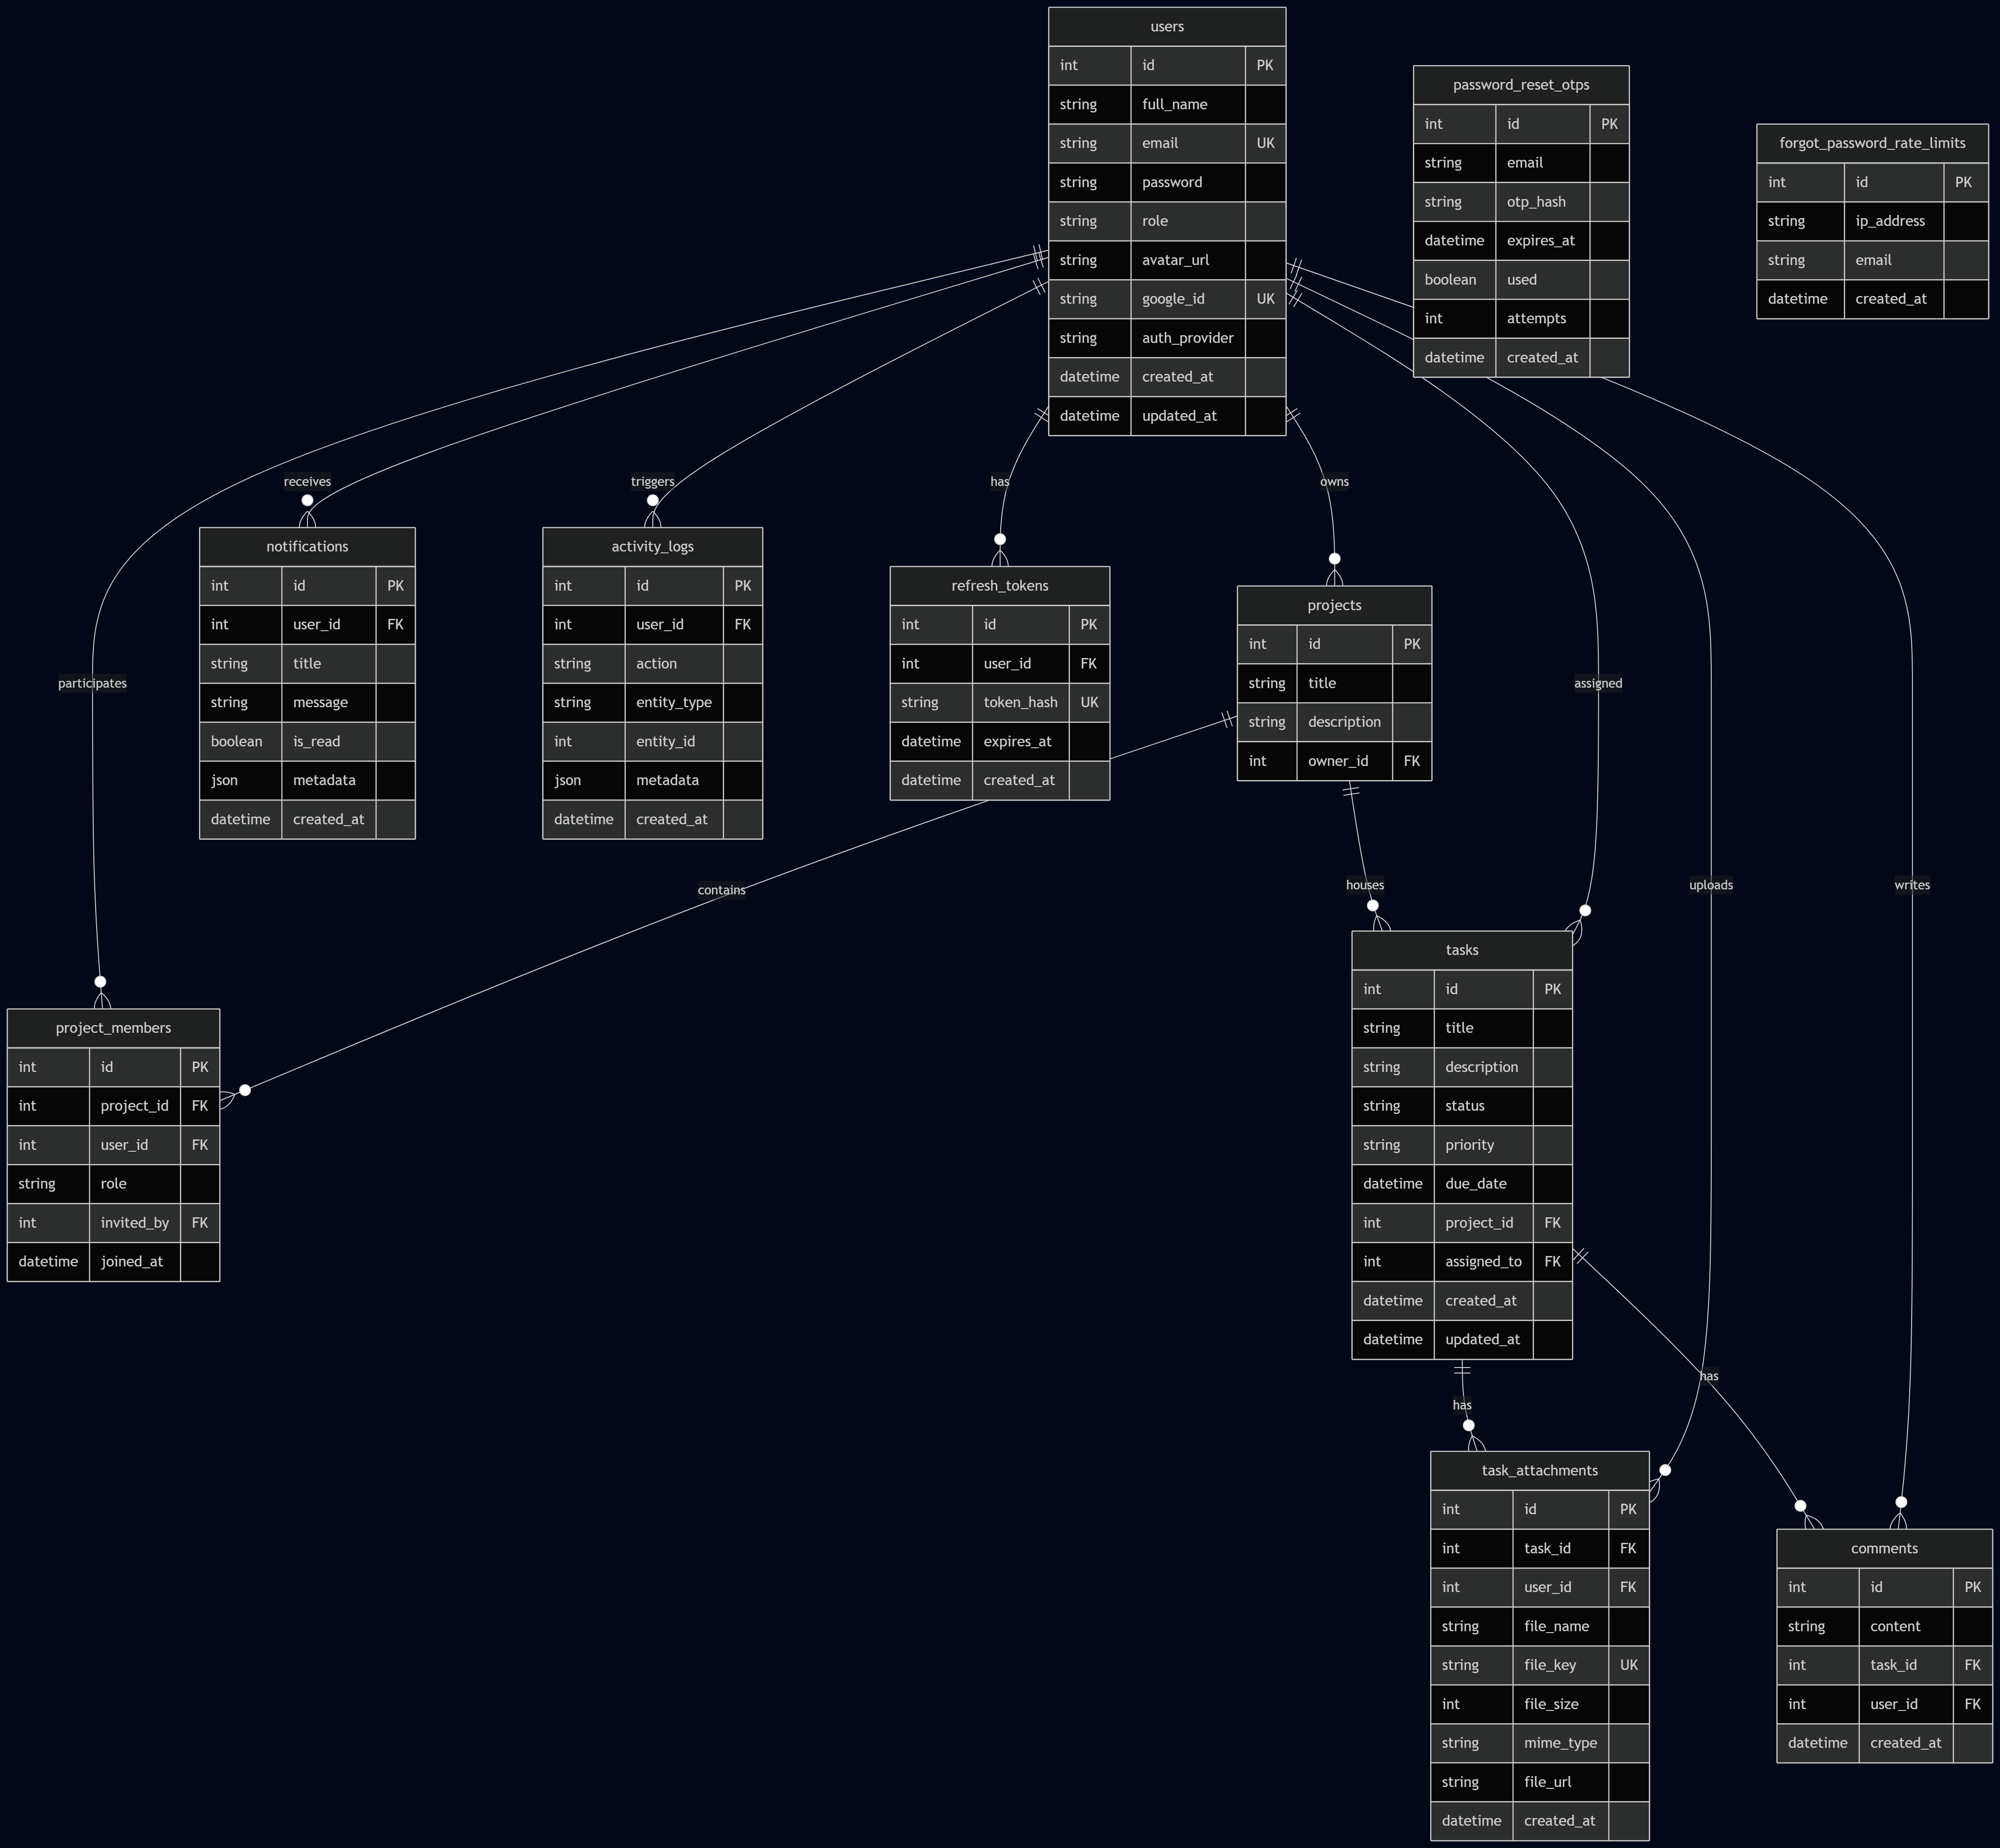
\includegraphics[width=\textwidth]{figures/database-erd.png}
    \caption{Nexus PM Relational Database Entity Relationship Diagram (ERD)}
    \label{fig:database_erd}
\end{figure}

The database models map to the following functional areas:
\begin{itemize}
    \item \textbf{Identity and Access:} \texttt{users} and \texttt{refresh\_tokens}.
    \item \textbf{Collaboration Boundaries:} \texttt{projects} and \texttt{project\_members}.
    \item \textbf{Core Task Engine:} \texttt{tasks}, \texttt{comments}, and \texttt{task\_attachments}.
    \item \textbf{Observability and Communications:} \texttt{notifications} and \texttt{activity\_logs}.
\end{itemize}

\pagebreak
\section{Table Descriptions}
The database tables are specified below.

\subsection{Users Table (\texttt{users})}
The \texttt{users} table stores credentials, Google OAuth profile linkages, and core system roles.

\begin{table}[h!]
\centering
\small
\renewcommand{\arraystretch}{1.4}
\begin{tabularx}{\textwidth}{l l l X}
    \toprule[1.5pt]
    \rowcolor{primary!5}
    \textbf{\color{primary}Column Name} & \textbf{\color{primary}Data Type} & \textbf{\color{primary}Constraints} & \textbf{\color{primary}Description} \\
    \midrule
    \texttt{id} & Integer & Primary Key, Index & Auto-incrementing identifier. \\
    \texttt{full\_name} & String(255) & Nullable=False & Full user name. \\
    \texttt{email} & String(255) & Unique, Index, Nullable=False & Core login identity parameter. \\
    \texttt{password} & String & Nullable=False & Hashed local user password. \\
    \texttt{role} & String(255) & Nullable=True & System role level. \\
    \texttt{avatar\_url} & Text & Nullable=True & Public CDN link to avatar graphic. \\
    \texttt{google\_id} & String(255) & Unique, Nullable=True & Google OAuth account identifier. \\
    \texttt{auth\_provider} & String(50) & Nullable=False, Default="local" & Provider type: "local" or "google". \\
    \texttt{created\_at} & DateTime & Nullable=False, Timezone=True & Record creation timestamp. \\
    \texttt{updated\_at} & DateTime & Nullable=False, Timezone=True & Record modification timestamp. \\
    \bottomrule[1.5pt]
\end{tabularx}
\caption{Users Table Schema Specification}
\label{tab:users_table}
\end{table}

\subsection{Projects Table (\texttt{projects})}
The \texttt{projects} table maps logical project workspaces.

\begin{table}[h!]
\centering
\small
\renewcommand{\arraystretch}{1.4}
\begin{tabularx}{\textwidth}{l l l X}
    \toprule[1.5pt]
    \rowcolor{primary!5}
    \textbf{\color{primary}Column Name} & \textbf{\color{primary}Data Type} & \textbf{\color{primary}Constraints} & \textbf{\color{primary}Description} \\
    \midrule
    \texttt{id} & Integer & Primary Key, Index & Auto-incrementing identifier. \\
    \texttt{title} & String & Nullable=False & Name of the project. \\
    \texttt{description} & String & Nullable=True & Serialized JSON for category, priority, and deadline metadata. \\
    \texttt{owner\_id} & Integer & Foreign Key (\texttt{users.id}) & Creator and owner user reference. \\
    \bottomrule[1.5pt]
\end{tabularx}
\caption{Projects Table Schema Specification}
\label{tab:projects_table}
\end{table}

\subsection{Project Members Table (\texttt{project\_members})}
This association table maps users to project workspaces, establishing roles and access permissions.

\begin{table}[h!]
\centering
\small
\renewcommand{\arraystretch}{1.4}
\begin{tabularx}{\textwidth}{l l l X}
    \toprule[1.5pt]
    \rowcolor{primary!5}
    \textbf{\color{primary}Column Name} & \textbf{\color{primary}Data Type} & \textbf{\color{primary}Constraints} & \textbf{\color{primary}Description} \\
    \midrule
    \texttt{id} & Integer & Primary Key, Index & Auto-incrementing identifier. \\
    \texttt{project\_id} & Integer & Foreign Key (\texttt{projects.id}), Cascade & Parent project reference. \\
    \texttt{user\_id} & Integer & Foreign Key (\texttt{users.id}), Cascade & Associated member reference. \\
    \texttt{role} & String(50) & Nullable=False, Default="viewer" & Permissions: owner, manager, developer, viewer. \\
    \texttt{invited\_by} & Integer & Foreign Key (\texttt{users.id}), Set Null & Inviting user reference. \\
    \texttt{joined\_at} & DateTime & Nullable=False, Timezone=True & Membership creation timestamp. \\
    \bottomrule[1.5pt]
\end{tabularx}
\caption{Project Members Table Schema Specification}
\label{tab:project_members_table}
\end{table}

\pagebreak
\subsection{Tasks Table (\texttt{tasks})}
The \texttt{tasks} table stores task details, assignments, status lanes, and due dates.

\begin{table}[h!]
\centering
\small
\renewcommand{\arraystretch}{1.4}
\begin{tabularx}{\textwidth}{l l l X}
    \toprule[1.5pt]
    \rowcolor{primary!5}
    \textbf{\color{primary}Column Name} & \textbf{\color{primary}Data Type} & \textbf{\color{primary}Constraints} & \textbf{\color{primary}Description} \\
    \midrule
    \texttt{id} & Integer & Primary Key, Index & Auto-incrementing identifier. \\
    \texttt{title} & String & Nullable=False & Brief task title. \\
    \texttt{description} & String & Nullable=True & Detailed task description. \\
    \texttt{status} & String & Default="TODO" & Kanban state: TODO, IN\_PROGRESS, REVIEW, DONE. \\
    \texttt{priority} & String & Default="MEDIUM" & Importance: LOW, MEDIUM, HIGH. \\
    \texttt{due\_date} & DateTime & Nullable=True, Timezone=True & Optional task deadline. \\
    \texttt{project\_id} & Integer & Foreign Key (\texttt{projects.id}) & Parent project reference. \\
    \texttt{assigned\_to} & Integer & Foreign Key (\texttt{users.id}), Nullable & Assigned user reference. \\
    \texttt{created\_at} & DateTime & Timezone=True & Record creation timestamp. \\
    \texttt{updated\_at} & DateTime & Timezone=True & Record modification timestamp. \\
    \bottomrule[1.5pt]
\end{tabularx}
\caption{Tasks Table Schema Specification}
\label{tab:tasks_table}
\end{table}

\subsection{Task Attachments Table (\texttt{task\_attachments})}
This table links uploaded file metadata to tasks.

\begin{table}[h!]
\centering
\small
\renewcommand{\arraystretch}{1.4}
\begin{tabularx}{\textwidth}{l l l X}
    \toprule[1.5pt]
    \rowcolor{primary!5}
    \textbf{\color{primary}Column Name} & \textbf{\color{primary}Data Type} & \textbf{\color{primary}Constraints} & \textbf{\color{primary}Description} \\
    \midrule
    \texttt{id} & Integer & Primary Key, Index & Auto-incrementing identifier. \\
    \texttt{task\_id} & Integer & Foreign Key (\texttt{tasks.id}), Cascade & Associated task reference. \\
    \texttt{user\_id} & Integer & Foreign Key (\texttt{users.id}), Set Null & Uploading user reference. \\
    \texttt{file\_name} & String(255) & Nullable=False & Original uploaded filename. \\
    \texttt{file\_key} & String(255) & Unique, Nullable=False & Unique S3 key within Cloudflare R2. \\
    \texttt{file\_size} & Integer & Nullable=False & Uploaded file size in bytes. \\
    \texttt{mime\_type} & String(100) & Nullable=False & MIME type of the file. \\
    \texttt{file\_url} & Text & Nullable=False & Target download URL address. \\
    \texttt{created\_at} & DateTime & Nullable=False, Timezone=True & File upload timestamp. \\
    \bottomrule[1.5pt]
\end{tabularx}
\caption{Task Attachments Table Schema Specification}
\label{tab:task_attachments_table}
\end{table}

\subsection{Comments Table (\texttt{comments})}
The \texttt{comments} table captures collaborative feedback threads linked to tasks.

\begin{table}[h!]
\centering
\small
\renewcommand{\arraystretch}{1.4}
\begin{tabularx}{\textwidth}{l l l X}
    \toprule[1.5pt]
    \rowcolor{primary!5}
    \textbf{\color{primary}Column Name} & \textbf{\color{primary}Data Type} & \textbf{\color{primary}Constraints} & \textbf{\color{primary}Description} \\
    \midrule
    \texttt{id} & Integer & Primary Key & Auto-incrementing identifier. \\
    \texttt{content} & Text & Nullable=False & Body content of the comment. \\
    \texttt{task\_id} & Integer & Foreign Key (\texttt{tasks.id}), Cascade, Index & Parent task reference. \\
    \texttt{user\_id} & Integer & Foreign Key (\texttt{users.id}), Cascade, Index & Comment author reference. \\
    \texttt{created\_at} & DateTime & Nullable=False, Timezone=True & Comment creation timestamp. \\
    \bottomrule[1.5pt]
\end{tabularx}
\caption{Comments Table Schema Specification}
\label{tab:comments_table}
\end{table}

\pagebreak
\subsection{Notifications Table (\texttt{notifications})}
This table stores in-app notification alerts.

\begin{table}[h!]
\centering
\small
\renewcommand{\arraystretch}{1.4}
\begin{tabularx}{\textwidth}{l l l X}
    \toprule[1.5pt]
    \rowcolor{primary!5}
    \textbf{\color{primary}Column Name} & \textbf{\color{primary}Data Type} & \textbf{\color{primary}Constraints} & \textbf{\color{primary}Description} \\
    \midrule
    \texttt{id} & Integer & Primary Key, Index & Auto-incrementing identifier. \\
    \texttt{user\_id} & Integer & Foreign Key (\texttt{users.id}), Cascade, Index & Target user reference. \\
    \texttt{title} & String(255) & Nullable=False & Subject title of the alert. \\
    \texttt{message} & Text & Nullable=False & Detailed description body. \\
    \texttt{is\_read} & Boolean & Nullable=False, Default=False & Flag for read status validation. \\
    \texttt{metadata} & JSON & Nullable=True & Optional payload (e.g. task ID, workspace ID). \\
    \texttt{created\_at} & DateTime & Nullable=False, Timezone=True & Generation timestamp. \\
    \bottomrule[1.5pt]
\end{tabularx}
\caption{Notifications Table Schema Specification}
\label{tab:notifications_table}
\end{table}

\subsection{Activity Logs Table (\texttt{activity\_logs})}
This table records project events to maintain an audit trail.

\begin{table}[h!]
\centering
\small
\renewcommand{\arraystretch}{1.4}
\begin{tabularx}{\textwidth}{l l l X}
    \toprule[1.5pt]
    \rowcolor{primary!5}
    \textbf{\color{primary}Column Name} & \textbf{\color{primary}Data Type} & \textbf{\color{primary}Constraints} & \textbf{\color{primary}Description} \\
    \midrule
    \texttt{id} & Integer & Primary Key, Index & Auto-incrementing identifier. \\
    \texttt{user\_id} & Integer & Foreign Key (\texttt{users.id}), Set Null, Index & Actor identity reference. \\
    \texttt{action} & String(255) & Nullable=False & Event code: CREATE, UPDATE, DELETE. \\
    \texttt{entity\_type} & String(255) & Nullable=False & Affected entity: Project, Task, Member. \\
    \texttt{entity\_id} & Integer & Nullable=True & Target record identifier. \\
    \texttt{metadata} & JSON & Nullable=True & Dynamic JSON changes payload. \\
    \texttt{created\_at} & DateTime & Nullable=False, Timezone=True & Logging execution timestamp. \\
    \bottomrule[1.5pt]
\end{tabularx}
\caption{Activity Logs Table Schema Specification}
\label{tab:activity_logs_table}
\end{table}

\subsection{Refresh Tokens Table (\texttt{refresh\_tokens})}
This table stores hashed refresh tokens to support session validation and revocation.

\begin{table}[h!]
\centering
\small
\renewcommand{\arraystretch}{1.4}
\begin{tabularx}{\textwidth}{l l l X}
    \toprule[1.5pt]
    \rowcolor{primary!5}
    \textbf{\color{primary}Column Name} & \textbf{\color{primary}Data Type} & \textbf{\color{primary}Constraints} & \textbf{\color{primary}Description} \\
    \midrule
    \texttt{id} & Integer & Primary Key, Index & Auto-incrementing identifier. \\
    \texttt{user\_id} & Integer & Foreign Key (\texttt{users.id}), Cascade, Index & User record reference. \\
    \texttt{token\_hash} & String(255) & Unique, Index, Nullable=False & Crytographic signature hash. \\
    \texttt{expires\_at} & DateTime & Nullable=False, Timezone=True & Expiration limit check. \\
    \texttt{created\_at} & DateTime & Nullable=False, Timezone=True & Token creation timestamp. \\
    \texttt{revoked} & Boolean & Nullable=False, Default=False & Revocation status flag. \\
    \bottomrule[1.5pt]
\end{tabularx}
\caption{Refresh Tokens Table Schema Specification}
\label{tab:refresh_tokens_table}
\end{table}

\subsection{Password Reset OTPs Table (\texttt{password\_reset\_otps})}
This table stores hashed verification OTP codes used for user registration activation and password reset operations.

\begin{table}[h!]
\centering
\small
\renewcommand{\arraystretch}{1.4}
\begin{tabularx}{\textwidth}{l l l X}
    \toprule[1.5pt]
    \rowcolor{primary!5}
    \textbf{\color{primary}Column Name} & \textbf{\color{primary}Data Type} & \textbf{\color{primary}Constraints} & \textbf{\color{primary}Description} \\
    \midrule
    \texttt{id} & Integer & Primary Key, Index & Auto-incrementing identifier. \\
    \texttt{email} & String(255) & Index, Nullable=False & Recipient user identity parameter. \\
    \texttt{otp\_hash} & String(64) & Nullable=False & Cryptographic verification code hash (SHA-256). \\
    \texttt{expires\_at} & DateTime & Nullable=False, Timezone=True & Expiration limit check. \\
    \texttt{used} & Boolean & Nullable=False, Default=False & Flag validating if OTP has been consumed. \\
    \texttt{attempts} & Integer & Nullable=False, Default=0 & Total verification retry counters. \\
    \texttt{created\_at} & DateTime & Nullable=False, Timezone=True & OTP generation timestamp. \\
    \bottomrule[1.5pt]
\end{tabularx}
\caption{Password Reset OTPs Table Schema Specification}
\label{tab:password_reset_otps_table}
\end{table}

\subsection{Forgot Password Rate Limits Table (\texttt{forgot\_password\_rate\_limits})}
This table logs password reset requests to protect authorization flows from brute-force attempts.

\begin{table}[h!]
\centering
\small
\renewcommand{\arraystretch}{1.4}
\begin{tabularx}{\textwidth}{l l l X}
    \toprule[1.5pt]
    \rowcolor{primary!5}
    \textbf{\color{primary}Column Name} & \textbf{\color{primary}Data Type} & \textbf{\color{primary}Constraints} & \textbf{\color{primary}Description} \\
    \midrule
    \texttt{id} & Integer & Primary Key, Index & Auto-incrementing identifier. \\
    \texttt{ip\_address} & String(45) & Index, Nullable=False & IP address of the client request. \\
    \texttt{email} & String(255) & Index, Nullable=False & Account email targeted by the request. \\
    \texttt{created\_at} & DateTime & Nullable=False, Timezone=True & Request logging timestamp. \\
    \bottomrule[1.5pt]
\end{tabularx}
\caption{Forgot Password Rate Limits Table Schema Specification}
\label{tab:forgot_password_rate_limits_table}
\end{table}

\pagebreak
\section{Relationships}
The Nexus PM schema models data dependencies using standard relational cardinality rules:
\begin{itemize}
    \item \textbf{One-to-One Relationships:} A user profile maps directly to active session entities in the \texttt{refresh\_tokens} table. When a user account is deleted, the corresponding session tokens are deleted via cascade rules.
    \item \textbf{One-to-Many Relationships:} Parent entities maintain logical ownership over dependent entities. Projects own multiple tasks, and tasks own multiple comments and attachments. Delete cascades are configured on these relationships (e.g., deleting a task automatically deletes its comments and attachment records).
    \item \textbf{Many-to-Many Relationships:} Users and projects have a many-to-many relationship, resolved by the \texttt{project\_members} association table. This table includes a unique constraint on \texttt{(project\_id, user\_id)} to prevent duplicate membership records.
    \item \textbf{Referential Integrity:} Foreign keys are protected using \texttt{ON DELETE CASCADE} for dependent resources and \texttt{ON DELETE SET NULL} for auditing and system history. For example, if a user is deleted, their entries in \texttt{activity\_logs} are preserved but anonymized by setting \texttt{user\_id} to null.
\end{itemize}

\section{Indexing Strategy}
To maintain fast response times as the database size increases, indexes are configured on frequently queried columns:
\begin{itemize}
    \item \textbf{Primary Keys:} PostgreSQL automatically creates unique B-Tree indexes on all primary key columns (\texttt{id}).
    \item \textbf{Unique Contraints:} Unique indexes are defined on \texttt{users(email)}, \texttt{users(google\_id)}, and \texttt{refresh\_tokens(token\_hash)} to ensure fast lookups and prevent duplicate records.
    \item \textbf{Foreign Keys:} Columns used in joins and filters (such as \texttt{project\_members(project\_id, user\_id)}, \texttt{tasks(project\_id)}, and \texttt{tasks(assigned\_to)}) are indexed to optimize Kanban board loads and workspace dashboards.
    \item \textbf{Search Indexes:} B-Tree indexes are configured on \texttt{comments(task\_id)} and \texttt{notifications(user\_id)} to speed up comments list loads and notifications retrieval.
\end{itemize}

\section{Transactions}
Relational operations are wrapped in database transactions to guarantee data consistency:
\begin{itemize}
    \item \textbf{Atomicity:} Complex workflows (e.g., project deletion, task state updates with audit logging) execute as a single atomic unit. If a step fails, the entire transaction is rolled back.
    \item \textbf{Read Committed Isolation:} The database uses the default Read Committed isolation level. This prevents dirty reads while allowing high concurrency.
    \item \textbf{Asynchronous Database Session Management:} The FastAPI backend manages database sessions asynchronously. Sessions are instantiated per request and closed automatically on request completion, returning the connection to the pool.
\end{itemize}

\section{Migration Strategy}
Schema evolution is managed using the \textbf{Alembic} migrations framework:
\begin{itemize}
    \item \textbf{Migration Scripts:} Database changes are written as versioned Python scripts inside the \path{alembic/versions/} directory.
    \item \textbf{Version Control:} Alembic tracks migrations using the \texttt{alembic\_version} table, which stores the current schema version hash.
    \item \textbf{Forward and Backward Migration:} Each script defines an \texttt{upgrade()} function to apply changes and a \texttt{downgrade()} function to revert them. This approach supports automated schema updates during CI/CD pipelines.
\end{itemize}

\section{Security}
Database security is enforced through configuration constraints:
\begin{itemize}
    \item \textbf{Row-Level validation:} Supabase Row-Level Security (RLS) is disabled by default to let PgBouncer handle connection routing directly. Read and write permissions are instead validated at the API layer.
    \item \textbf{Hashed Credentials:} Plaintext user passwords are never saved. The application hashes passwords using bcrypt before saving them to the database.
    \item \textbf{Input Validation Constraints:} Column length constraints (e.g., \texttt{String(255)} for email values) are enforced at both the SQLAlchemy model layer and database schema layer, preventing buffer overflow vulnerabilities.
\end{itemize}

\section{Scalability}
The database design incorporates several optimizations to support system scaling:
\begin{itemize}
    \item \textbf{PgBouncer Connection Pooling:} Supabase handles connection routing through PgBouncer, resolving database connection limits. The engine disables the local statement cache (\texttt{"statement\_cache\_size": 0}) to avoid conflicts with PgBouncer's transaction mode.
    \item \textbf{JSON Columns for Metadata:} Columns like \texttt{projects.description} and \texttt{notifications.metadata} use JSON fields to store non-searchable, semi-structured metadata, reducing the need for schema changes.
    \item \textbf{Read and Write Segregation:} Decoupled model queries allow for future read-write segregation, where read traffic can be routed to read-only database replicas.
\end{itemize}

\section{Chapter Summary}
This chapter detailed the database design for Nexus PM. By defining table schemas, indexing strategies, relationship mappings, and transactional boundaries, the design provides a reliable data persistence layer. The database design supports workspace isolation, secure session tracking, and fast query execution. The next chapter will build on these blueprints, detailing the REST API endpoints and data validation flows.
